
\documentclass{beamer}
\usepackage[utf8]{inputenc}
\usepackage{multicol}
\usepackage{amsmath}
\usepackage[english]{babel}
\usepackage{algorithm}
\usepackage[noend]{algpseudocode}

\begin{document}
\begin{frame}

    \frametitle{Problema 1}
    \begin{algorithm}[H]
        \caption{HeapSort}
        \begin{algorithmic}[1]
        \Procedure{HEAPSORT}{$A$}
        \State BUILD-MAX-HEAP()
        
        	\For{$i\gets 1\ \mathbf{to}\ len(A) - 1$}
		\For{$j\gets 2\ \mathbf{to}\ len(A) - 1$}
			\If{$ A[i] <= A[j] $ }
				\State {$min\gets A[j]$}
			\EndIf	
		\EndFor
		\State newArr [i] = min 
	\EndFor
	\EndProcedure
        \end{algorithmic}
    \end{algorithm}
    \textbf{running-time:} es peor que el HeapSort porque su complejidad es de O( $n^2$ ) 
    \end{frame}

\begin{frame}
\frametitle{Problema 2}
\textbf{1.)} O( $n * log (n) $ ) \newline


\textbf{3.)}  El HeapSort siempre será complejidad de  n log(n), sin embargo el Quicksort tiene la ventaja de hacer swaps necesarios, no como el HeapSort que siempre rompe la propiedad de heap y la vuelve a construir. En el Quicksort también se tiene la ventaja de elegir un buen pivot y posiblemente ahorre trabajo de partición o casualmente el pivote elegido es un valor intermedio de los valores. 

\end{frame}
\begin{frame}
\frametitle{Problema 2}
\textbf{2.)}      \newline
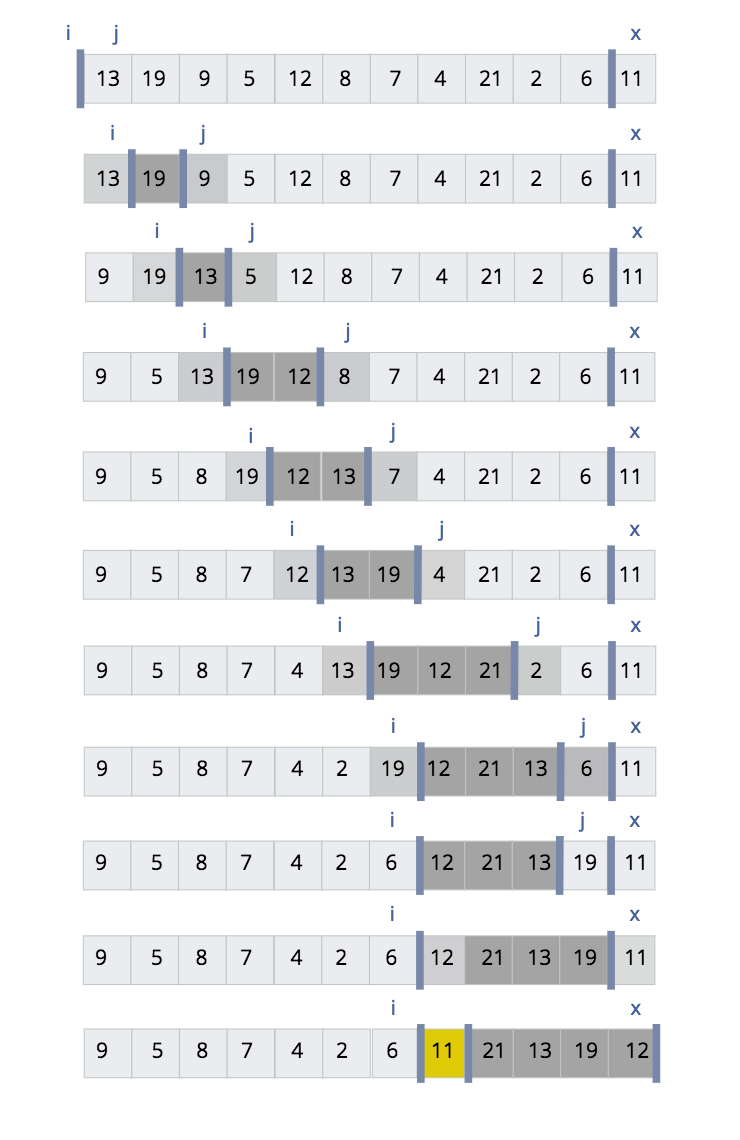
\includegraphics[width=5.5cm]{partition.jpg}

\end{frame}
\begin{frame}
\frametitle{Problema 3}
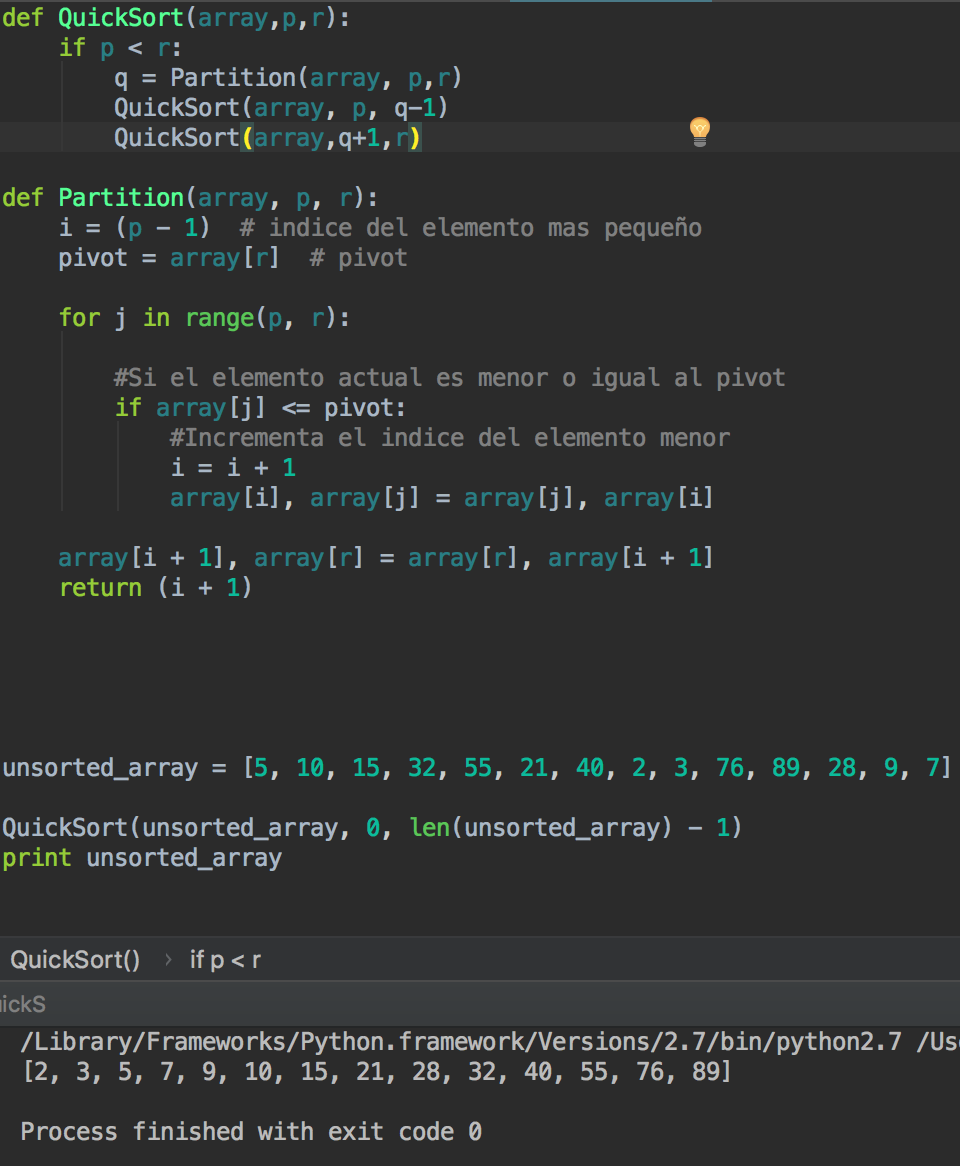
\includegraphics[width=7cm]{quick.png}
\end{frame}

\end{document}





